% !TEX program = xelatex
\documentclass[11pt,a4paper]{article}
\usepackage[margin=2.1cm]{geometry}
\usepackage{fontspec}
\usepackage{microtype}
\usepackage{booktabs}
\usepackage{tabularx}
\usepackage{array}
\usepackage{xcolor}
\usepackage{enumitem}
\usepackage{caption}
\usepackage{float}
\usepackage{pgfplots}
\pgfplotsset{compat=1.18}
\usepackage[hidelinks]{hyperref}

% ---------- palette (same as Battlecode ladder strategy analysis.tex) ----------
\definecolor{cTop}{HTML}{2B6CB0}
\definecolor{cMid}{HTML}{9F7AEA}
\definecolor{cLow}{HTML}{A0AEC0}
\definecolor{cOurs}{HTML}{D9480F}
\definecolor{cOpp}{HTML}{2F855A}
\definecolor{cGood}{HTML}{2F855A}
\definecolor{cBad}{HTML}{C53030}
\definecolor{cInk}{HTML}{2D3748}
\definecolor{cSoft}{HTML}{EDF2F7}

% ---------- source / code macros ----------
\newcommand{\data}{file:///Users/tristanbasri/Desktop/Code/battlecode-scrim-2026-10-25}
\newcommand{\repo}{file:///Users/tristanbasri/Desktop/Code/cambridge-battlecode-s2}
% \src{url}{label}: inline source citation
\newcommand{\src}[2]{{\small(\href{#1}{\textcolor{cTop}{\texttt{#2}}})}}
% \code{repo-relative-path}{display}: clickable code reference to our bot
\newcommand{\code}[2]{\href{\repo/#1}{\texttt{\textcolor{cOurs!80!black}{#2}}}}
\newcommand{\veight}{bots/bot-v8/src}
\newcommand{\HP}{\textbf{HP}}

\setlength{\parskip}{0.45em}
\setlength{\emergencystretch}{2em}
\setlength{\parindent}{0pt}
\captionsetup{font=small,labelfont=bf}
\setlist{itemsep=0.25em,topsep=0.3em}

\title{\vspace{-1.2cm}\textbf{bot-v8 against the top 100: where we lose and why}\\[0.3em]
\large 485 scrims against the top 100, 747 recent ranked games of the top 100,\\ and 3,642 ranked games from the 24 October match-database dump}
\author{Research report on ladder data from 2026-10-24 and 2026-10-25}
\date{25 October 2026}

\begin{document}
\maketitle

\noindent\colorbox{cSoft}{\parbox{\dimexpr\linewidth-2\fboxsep}{\small
\textbf{Bottom line.} bot-v8 won \textbf{104 of 485 scrims} against the top 100 (21\%, 95\% CI 18--25\%), from a ladder position of about \#94--\#100. There are \textbf{two cliffs}. We win 40\% against ranks 81--100, about 23\% against ranks 31--80, and \textbf{4\%} against ranks 1--30. We lose on \textbf{economy, and the gap shows up early}: in losses we are 82 gold behind at round 100, 411 at round 300 and 2,573 at round 1000. The team ahead on gold at round 300 wins about 73\% of top-100 ranked games. v8 \textbf{funnels camp captures to Vesper Vale}, so our Marcella, Heart of Ruin and Vendetta earn only \textbf{41--65\%} of the gold the same champions earn on the other side. We also \textbf{die more} (13 deaths a game against 8), our builds \textbf{stack one stat}, and we \textbf{run out of fuel on about 140 turns a game}, against 10--15 for top teams. The draft is not the problem: we draft the same core as the top 30. A local A/B (Section~\ref{sec:fix}) then showed that turning the funnel off \emph{lowers} team gold, and that Health builds give no reliable gain, so the gold gap's real cause is still open.}}

\vspace{0.6em}
{\small\textbf{Data windows.} The \emph{scrims} are 97 unranked 5-game groups of bot-v8 against the top-100 teams, queued from 24 Oct 00:14 to 25 Oct 11:20 with maps cycled and sides alternated \src{\data/scrim/groups.jsonl}{scrim/groups.jsonl}. The \emph{top-100 sample} is each team's 15 most recent ranked games, pulled with \texttt{cambc matches summary} \src{\data/scrim/rows\_top.jsonl}{scrim/rows\_top.jsonl}. The \emph{match-database check} uses parts 1--2 of the organiser's 24 Oct summary dump: 49,535 matches, of which 3,642 are ranked games involving a top-100 team \src{\data/matchdb/}{matchdb/}. All three go through the same feature code. Full tables are in the companion file \texttt{v8\_ladder\_scrim\_tables.tex}.}

\tableofcontents

%=====================================================================
\section{Where we start losing}
%=====================================================================

Ranks are the opponent's rank when the group was queued. Each team got one 5-game group.

\begin{figure}[H]
\centering
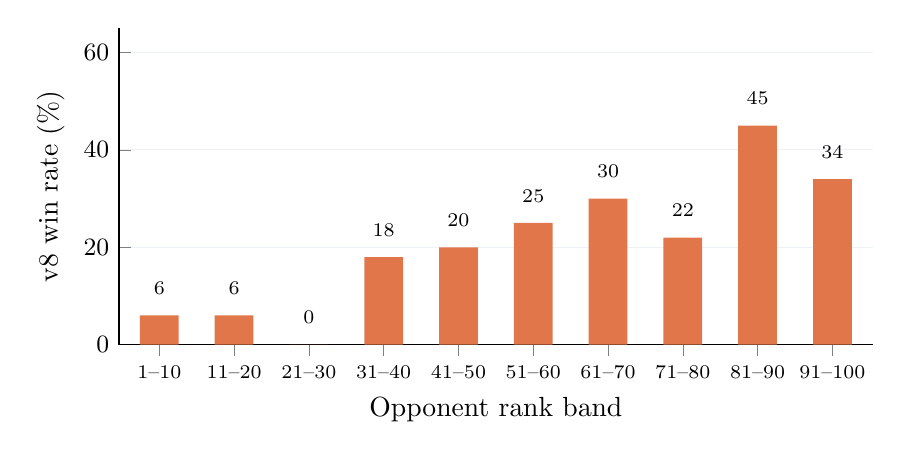
\begin{tikzpicture}
\begin{axis}[
  width=0.92\linewidth, height=5.6cm,
  ybar, bar width=14pt,
  ymin=0, ymax=65,
  ylabel={v8 win rate (\%)},
  xlabel={Opponent rank band},
  symbolic x coords={1--10,11--20,21--30,31--40,41--50,51--60,61--70,71--80,81--90,91--100},
  xtick=data,
  x tick label style={font=\scriptsize},
  y tick label style={font=\small},
  ymajorgrids, grid style={cSoft},
  axis lines*=left,
  nodes near coords, nodes near coords style={font=\scriptsize, above=4pt},
  enlarge x limits=0.06,
]
\addplot[fill=cOurs!75, draw=none] coordinates {
  (1--10,6)
  (11--20,6)
  (21--30,0)
  (31--40,18)
  (41--50,20)
  (51--60,25)
  (61--70,30)
  (71--80,22)
  (81--90,45)
  (91--100,34)
};
\end{axis}
\end{tikzpicture}
\caption{bot-v8 scrim win rate by opponent rank band (40--60 games per band). The two drops are at about rank 80 and at rank 30. Confidence intervals are in Table~\ref{tab:bands}.}
\label{fig:bands}
\end{figure}

\begin{table}[H]
\centering\footnotesize\setlength{\tabcolsep}{5pt}
\begin{tabular}{lrrlll}
\toprule
Opponent rank & Games & Our wins & Win rate [95\% CI] & Gems tributed, us / them & Gold@300, us / them \\
\midrule
1--10   & 50 & 3  & 6\% [2--16\%]   & 351 / 994   & 1,048 / 1,496 \\
11--20  & 50 & 3  & 6\% [2--16\%]   & 350 / 1,017 & 1,042 / 1,497 \\
21--30  & 40 & 0  & 0\% [0--9\%]    & 315 / 1,114 & 983 / 1,671 \\
\midrule
31--40  & 45 & 8  & 18\% [9--31\%]  & 472 / 931   & 1,014 / 1,379 \\
41--50  & 50 & 10 & 20\% [11--33\%] & 541 / 886   & 1,154 / 1,418 \\
51--60  & 40 & 10 & 25\% [14--40\%] & 565 / 903   & 1,136 / 1,298 \\
61--70  & 50 & 15 & 30\% [19--44\%] & 681 / 845   & 1,153 / 1,122 \\
71--80  & 50 & 11 & 22\% [13--35\%] & 548 / 910   & 1,003 / 1,215 \\
\midrule
81--90  & 60 & 27 & 45\% [33--58\%] & 724 / 771   & 1,216 / 1,272 \\
91--100 & 50 & 17 & 34\% [22--48\%] & 632 / 816   & 1,101 / 1,176 \\
\bottomrule
\end{tabular}
\caption{Scrim results by opponent rank band \src{\data/scrim/report\_final.md}{scrim/report\_final.md}.}
\label{tab:bands}
\end{table}

\begin{itemize}
  \item \textbf{Ranks 81--100 are our peers.} Games against them are close: gems tributed are within about 10--20\%, and gold at round 300 is within 5\%.
  \item \textbf{Around rank 80 we lose about half our win rate.} From there to rank 31 the win rate is flat at about 20--30\%, and the gold gap at round 300 grows to 200--400.
  \item \textbf{Above rank 30 the top teams beat us in about 96\% of games.} By round 300 they are 450--700 gold ahead, and they end with three times our tributed gems. Gains in the 31--80 band are realistic for the next version; the top 30 needs a much stronger economy.
  \item \textbf{A logistic fit on rating} puts our 50\% point at about rating 1742, which is our own level, and our 30\% point at about rating 1853 ($\approx$ rank 74).
\end{itemize}

%=====================================================================
\section{Both sides of the same games}
%=====================================================================

Table~\ref{tab:losses} averages our 381 losses; the opponent's numbers come from the same games.

\begin{table}[H]
\centering\small
\begin{tabular}{lrrr}
\toprule
Metric & v8 & Opponent & Gap \\
\midrule
Gold earned @100          & 285   & 367   & $-82$ \\
Gold earned @300          & 1,009 & 1,420 & $-411$ \\
Gold earned @1000         & 4,281 & 6,854 & $-2{,}573$ \\
Gems tributed @1000       & 288   & 582   & $-294$ \\
Camp clears               & 53    & 63    & $-10$ \\
Kills / deaths            & 3.9 / 15 & 14 / 5.2 & \\
Gems per tribute          & 31    & 52    & $-21$ \\
Wards placed              & 142   & 200   & $-58$ \\
Altar locks bought        & 8.4   & 4.1   & $+4.3$ \\
Teleport crystals bought  & 0     & 5.5   & $-5.5$ \\
Fuel-exhausted turns      & 140   & 13    & $+127$ \\
Unspent gold at end       & 222   & 769   & $-547$ \\
\bottomrule
\end{tabular}
\caption{v8 against the opponent in our 381 scrim losses.}
\label{tab:losses}
\end{table}

In our 104 wins the picture flips. We lead on gold from round 100 (373 against 319), clear more camps (80 against 52), and get 16 kills to their 6. \textbf{The games are decided by who farms better in the first 300 rounds, and the fights follow from that.}

\subsection{The funnel starves four of our five champions}

Table~\ref{tab:samechamp} compares the same champion on both sides, in scrims where both teams drafted it.

\begin{figure}[H]
\centering
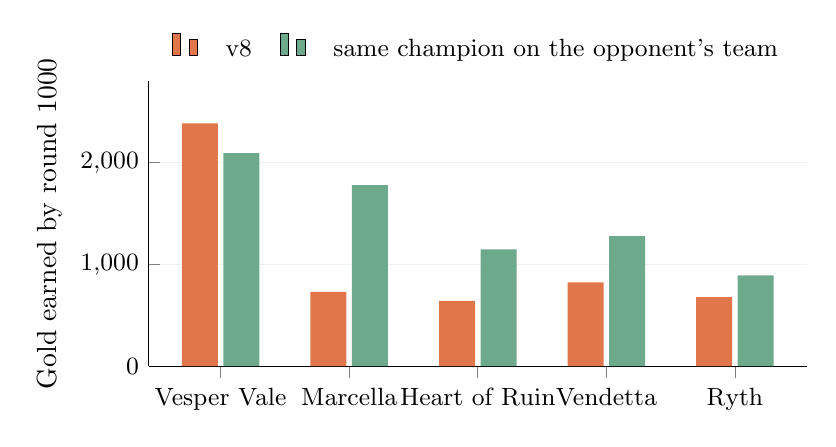
\begin{tikzpicture}
\begin{axis}[
  width=0.82\linewidth, height=5.2cm,
  ybar, bar width=13pt,
  ymin=0, ymax=2800,
  ylabel={Gold earned by round 1000},
  symbolic x coords={Vesper Vale,Marcella,Heart of Ruin,Vendetta,Ryth},
  xtick=data,
  x tick label style={font=\small},
  y tick label style={font=\small},
  ymajorgrids, grid style={cSoft},
  axis lines*=left,
  legend style={font=\small, draw=none, at={(0.5,1.03)}, anchor=south, legend columns=2, column sep=8pt},
  legend cell align=left,
  enlarge x limits=0.14,
  scaled y ticks=false,
]
\addplot[fill=cOurs!75, draw=none] coordinates {(Vesper Vale,2386) (Marcella,731) (Heart of Ruin,642) (Vendetta,824) (Ryth,679)};
\addplot[fill=cOpp!70, draw=none] coordinates {(Vesper Vale,2093) (Marcella,1779) (Heart of Ruin,1149) (Vendetta,1277) (Ryth,892)};
\legend{v8, same champion on the opponent's team}
\end{axis}
\end{tikzpicture}
\caption{Gold earned by round 1000, same champion on both sides. Only our Vesper out-earns her counterpart.}
\label{fig:samechamp}
\end{figure}

\begin{table}[H]
\centering\footnotesize\setlength{\tabcolsep}{5pt}
\begin{tabular}{lrrrrrr}
\toprule
Champion & Games & v8 gold@300 & Opp gold@300 & v8 gold@1000 & Opp gold@1000 & v8 share @1000 \\
\midrule
Vesper Vale   & 427 & 527 & 462 & 2,386 & 2,093 & \textcolor{cGood}{114\%} \\
Marcella      & 419 & 157 & 375 & 731   & 1,779 & \textcolor{cBad}{41\%} \\
Heart of Ruin & 353 & 145 & 257 & 642   & 1,149 & \textcolor{cBad}{56\%} \\
Vendetta      & 301 & 171 & 259 & 824   & 1,277 & \textcolor{cBad}{65\%} \\
Ryth          & 226 & 153 & 184 & 679   & 892   & 76\% \\
\bottomrule
\end{tabular}
\caption{Same-champion economy in scrims \src{\data/scrim/deep\_final.md}{scrim/deep\_final.md}.}
\label{tab:samechamp}
\end{table}

\begin{itemize}
  \item \textbf{Vesper gains about 65 gold at round 300; the other four lose 30--220 each.} Overall the team ends up about 400 behind at round 300, which matches the deficit in our losses.
  \item \textbf{This comes from the capture funnel in \code{\veight/common/camps.rs}{camps.rs}.} With \texttt{FUNNEL\_MELEE} on (\code{\veight/common/camps.rs}{camps.rs:241}), Bruisers (Marcella, Heart of Ruin) and Assassins (Vendetta) leave a cleared camp's capture to Vesper, the gold-bonus carry. \texttt{TANK\_FUNNEL} (\code{\veight/common/camps.rs}{camps.rs:10}) does the same for Ryth, a Tank. Those are exactly the starved champions: the three \texttt{FUNNEL\_MELEE} classes are at 41--65\%, and Ryth is at 76\%. (The Group opening's \texttt{GROUP\_FUNNEL} in \texttt{opening.rs} is inactive in v8, because \texttt{GROUP\_MODE = false}.) Concentrating gold on Vesper should pay off because of her +53\% gold passive with Treasure. In practice the team as a whole farms less: in losses we clear 10 fewer camps, and the others have far fewer items. A 2026-10-24 local test against our own bot had \texttt{FUNNEL\_MELEE} off at 109/200 against a 97/200 control, within noise (\code{\veight/common/rally.rs}{rally.rs:721}).
  \item \textbf{The others end up with far fewer emblems.} Our Marcella completes 6.4 emblems a game against 12 for top-30 Marcellas. Our Heart of Ruin completes 5.2 against 7.9, and our Vendetta 6.5 against 9.4. Our Vesper completes 20 against 14.
\end{itemize}

\subsection{We die about 1.6\texorpdfstring{$\times$}{x} as often, and every champion is affected}

\begin{table}[H]
\centering\footnotesize\setlength{\tabcolsep}{4pt}
\begin{tabular}{lrrrr}
\toprule
 & v8 & Scrim opp. & Top-100 & Ranks 1--30 \\
\midrule
Deaths per game            & 13  & 8.0 & 9.3 & 9.3 \\
Killed by champions        & 12  & 6.7 & 8.1 & 8.4 \\
Deaths before round 300    & 2.0 & 1.5 & 1.8 & 1.9 \\
Median first death (round) & 139 & 172 & 160 & 164 \\
\bottomrule
\end{tabular}
\quad
\begin{tabular}{lrr}
\toprule
v8 champion & Deaths/game & Opp.\ same champion \\
\midrule
Vendetta      & 3.5 & 1.9 \\
Heart of Ruin & 3.0 & 1.9 \\
Marcella      & 3.0 & 1.5 \\
Ryth          & 2.8 & 1.9 \\
Vesper Vale   & 2.2 & 1.4 \\
\bottomrule
\end{tabular}
\caption{Deaths: v8 against scrim opponents and top-100 ranked play (left), and by champion (right).}
\end{table}

\begin{itemize}
  \item \textbf{Who kills us:} opponent Marcella gets 27\% of our deaths, Vesper 21\%, Heart of Ruin 15\% and Vendetta 15\%. Camps cause only 8\%. We lose fights against the same comp we draft.
  \item \textbf{Vesper loses the most gems on death,} 52 a game. She carries the funnelled gems, and each death hands them to the killer.
\end{itemize}

\subsection{Builds: we stack one stat, the top teams mix}

Table~\ref{tab:builds} shows the purchase order of the first three emblems, and the share of all completed emblems by stat. v8 builds are fixed, so its rows are 100\% one order.

\begin{table}[H]
\centering\footnotesize
\begin{tabularx}{\linewidth}{l>{\raggedright\arraybackslash}X>{\raggedright\arraybackslash}X>{\raggedright\arraybackslash}p{2.2cm}>{\raggedright\arraybackslash}p{2.4cm}}
\toprule
Champion & v8 first three & Most common top-30 first three & Stat mix, v8 & Stat mix, ranks 1--30 \\
\midrule
Vesper Vale & Treasure Str $\to$ Bruiser Str $\to$ Durability HP & Treasure Str $\to$ Jungle Str $\to$ Bruiser \HP{} (31\%) & Str 95\%, HP 5\% & Str 73\%, HP 27\% \\
Marcella & Treasure HP $\to$ Jungle HP $\to$ Bruiser Str & Treasure HP $\to$ Jungle Str $\to$ Bruiser HP (20\%); several \textbf{Focus} lines & Str 65\%, HP 35\%, \textbf{Focus 0\%} & \textbf{Focus 41\%}, HP 35\%, Str 25\% \\
Vendetta & Treasure Str $\to$ Jungle Str $\to$ Bruiser Str & Treasure \HP{} $\to$ Jungle Str $\to$ Bruiser \HP{} (39\%) & Str 91\%, HP 9\% & Str 61\%, HP 39\% \\
Heart of Ruin & Treasure Focus $\to$ Jungle Focus $\to$ Bruiser Focus & Treasure \HP{} $\to$ Jungle Focus $\to$ Bruiser \HP{} (24\%) & Focus 89\%, HP 11\% & Focus 62\%, HP 37\% \\
Ryth & Treasure HP $\to$ Jungle HP $\to$ Bruiser HP & Treasure HP $\to$ Jungle \textbf{Str} $\to$ Bruiser HP (44\%) & HP 100\% & HP 55\%, Str 44\% \\
\bottomrule
\end{tabularx}
\caption{Emblem builds: v8 against ranks 1--30 (ranked games).}
\label{tab:builds}
\end{table}

\begin{itemize}
  \item \textbf{Marcella builds differ, but it may not matter.} Her slot-1 spell deals $2\times$ Focus, and Focus grows +15 per shard against +5 Strength (\code{docs/GameRules.md}{GameRules.md}, Marcella). Top teams build her Focus-first in many games, while v8 builds no Focus at all (\code{\veight/champions/marcella.rs}{marcella.rs:16}). However, in the match-database sample Focus Marcella builds don't win more than other builds (Section~\ref{sec:db}).
  \item \textbf{Vesper and Vendetta are glass cannons.} Both builds repeat Bruiser Strength once the list runs out (\code{\veight/champions/vesper\_vale.rs}{vesper\_vale.rs:13}, \code{\veight/champions/vendetta.rs}{vendetta.rs:13}; \code{\veight/bot.rs}{bot.rs:158} repeats the last entry). That fits their 1.5--1.8$\times$ death rate. Top teams take a Health emblem early, most often a third-emblem Bruiser Health.
  \item \textbf{Ryth goes all-Health;} top teams mix in Strength (Jungle Strength second in 44\% of top-30 games).
\end{itemize}

\subsection{Fuel: about 10\texorpdfstring{$\times$}{x} more lost turns}

\begin{table}[H]
\centering\small
\begin{tabular}{lrrrrr}
\toprule
 & Per game & During combat & Rounds 0--100 & 100--500 & 500+ \\
\midrule
v8                & 140 & 17 (12\%) & 20  & 48  & 72 \\
Scrim opponents   & 13  & 1.1       & 4.3 & 3.3 & 5.3 \\
Ranks 1--30 ranked & 12 & 0.9       & 7.8 & 2.1 & 1.7 \\
\bottomrule
\end{tabular}
\caption{Fuel-exhausted turns per game (team total). ``During combat'' means the champion took champion damage within 3 rounds.}
\end{table}

\begin{itemize}
  \item \textbf{Every v8 champion stalls; it isn't one bad script.} Per game: Vendetta 39, Heart of Ruin 35, Ryth 33, Marcella 28, Vesper 22.
  \item \textbf{When fuel runs out, the champion's turn is suspended and resumes next round} (\code{docs/GameRules.md}{GameRules.md}, Fuel). About 2\% of our champion-turns are lost, mostly while farming or walking. That is a small but steady drag on economy.
  \item \textbf{Within our own games, fuel stalls barely track the result.} We win 26\% with under 50 stalls and 18--22\% with more. Fixing fuel is worth doing, but on its own it won't close the gap.
\end{itemize}

\subsection{Maps}

Each map has 11--14 games, so treat these as hints. We are 0--1 wins on \textbf{00interlock, 01shortcut, 01elk\_arena, 00expanse, 01gold\_rush and 00lost\_world}. We are 43--50\% on \textbf{00contest, 00gemfight, 00fragment, 00elkring and 00rushbait\_v2}. Side barely matters: 23\% on side A, 20\% on side B.

%=====================================================================
\section{What the top 100 do (747 recent ranked games)}
%=====================================================================

\begin{itemize}
  \item \textbf{Comps have settled on one core,} the same one we draft. Vesper Vale is in 84--90\% of comps, Marcella 81--88\%, Heart of Ruin 70--81\% and Vendetta 62--70\%; Ryth is 47--76\%. The most common top-30 comp is Heart of Ruin/Marcella/Ryth/Vendetta/Vesper (116 team-games, 51\% win rate). \textbf{The draft is not where we lose.}
  \item \textbf{Gold decides games.} In top-100 games the gold leader wins 61\% at round 100, 74\% at round 300, 77\% at round 500 and 85\% at round 1000. Winners have more gold than the loser at round 1000 in 85\% of games. Kills, camp clears and gems per tribute come next (66--74\%).
  \item \textbf{Winners die less:} 5.5 deaths a game against 13 for losers.
  \item \textbf{Top teams barely run out of fuel:} 12--15 stalls a game, mostly in the first 100 rounds, likely during setup.
  \item \textbf{Teleport crystals:} 29\% of top-100 team-games buy at least one (4.7 per team-game in ranks 1--30), mostly Marcella and Vesper, at a median of round 533. They don't predict winning (48\% win rate with, 52\% without), so they're low priority.
  \item \textbf{Altar locks:} top teams buy 4--5 a game against our 8--9. Winners and losers buy the same number.
  \item \textbf{Builds:} top-30 teams spread emblems across Bruiser Strength, Bruiser Health and Bruiser Focus (15 / 11 / 5 per team-game for ranks 1--10). Our builds put almost everything into one stat per champion (Table~\ref{tab:builds}).
\end{itemize}

%=====================================================================
\section{Match-database check: 3,642 ranked games from 24 October}
\label{sec:db}
%=====================================================================

This section uses \texttt{summaries-2026-10-24-part1.zip} and \texttt{part2.zip} from the site's match database: 49,535 matches, of which 3,642 are ranked games involving a top-100 team. That is 4.9$\times$ the sample in the previous section, run through the same feature code \src{\data/matchdb/report\_db.md}{matchdb/report\_db.md}, \src{\data/matchdb/deep\_db.md}{matchdb/deep\_db.md}.

\textbf{Everything in the previous section replicates.}

\begin{table}[H]
\centering\footnotesize\setlength{\tabcolsep}{5pt}
\begin{tabular}{lll}
\toprule
 & \texttt{cambc} sample (747) & Match database (3,642) \\
\midrule
P(gold leader wins) @300 / @1000 & 74\% / 85\% & 73\% / 83\% \\
Winner deaths / loser deaths & 5.5 / 13 & 5.7 / 14 \\
Fuel-exhausted turns, ranks 1--30 & 12 & 10 \\
Deaths per game, ranks 1--30 & 9.3 & 8.8 \\
Most common top-30 comp$^{*}$ & core five (51\%) & core five (441 games, 53\%) \\
Top-30 stat mix, Vesper / Vendetta & Str 73/61\%, HP 27/39\% & Str 73/62\%, HP 27/38\% \\
Crystals: win rate with / without & 48\% / 52\% & 52\% / 50\% \\
\bottomrule
\end{tabular}
\caption{Replication of the top-100 findings on the match-database dump. $^{*}$Core five: Heart of Ruin, Marcella, Ryth, Vendetta, Vesper Vale.}
\end{table}

\textbf{Do the top teams' build choices actually win more?} Table~\ref{tab:buildwin} compares top-100 team-games by how many of a champion's first four emblems are of one stat. It only covers champions that completed at least three emblems, which is why all the rates are above 50\%.

\begin{table}[H]
\centering\footnotesize\setlength{\tabcolsep}{4pt}
\begin{tabular}{llll}
\toprule
Champion (stat counted) & 0 of that stat & 1 & 2 or more \\
\midrule
Vesper Vale (Health)   & 54\% (n=169)   & 53\% (n=2,215) [51--55] & \textbf{56\%} (n=2,458) [54--58] \\
Vendetta (Health)      & 46\% (n=50)    & 53\% (n=975) [50--56]   & \textbf{57\%} (n=2,525) [55--59] \\
Heart of Ruin (Health) & 62\% (n=116)   & 52\% (n=1,000) [49--55] & 56\% (n=2,740) [55--58] \\
Ryth (Strength)        & 56\% (n=409)   & 56\% (n=1,542) [54--59] & 59\% (n=1,062) [56--62] \\
Marcella (Focus)       & 57\% (n=1,986) [55--59] & 53\% (n=731) [49--57] & 56\% (n=1,995) [54--58] \\
\bottomrule
\end{tabular}
\caption{Win rate by build stat mix among the first four emblems, top-100 ranked team-games, with 95\% Wilson intervals.}
\label{tab:buildwin}
\end{table}

\begin{itemize}
  \item \textbf{Health on Vesper and Vendetta has the clearest link to winning, but it's modest:} about +3--4 points over one Health emblem, with confidence intervals that barely overlap. Part 1 alone showed +6; adding part 2 shrank it. v8 builds take zero or one Health emblem among the first four.
  \item \textbf{Heart of Ruin} shows a similar +4 for two or more Health emblems over one.
  \item \textbf{Marcella Focus shows no benefit.} That lowers its priority in Section~\ref{sec:fix}.
  \item \textbf{Ryth's mixed Strength build} trends slightly upward. None of these build effects is large; the economy gap (Table~\ref{tab:samechamp}) is far bigger.
  \item \textbf{This is still correlation:} builds also reflect the rest of each bot. Treat it as evidence for which A/B tests to run first.
\end{itemize}

%=====================================================================
\section{What to change, in order}
\label{sec:fix}
%=====================================================================

The first two candidates were A/B tested locally on 2026-10-25; neither won. 312-game A/B noise is about $\pm$20 wins.

\subsection*{Local A/B results}

Each variant played 624 games against bot-v8 (52 maps $\times$ 2 sides $\times$ 6 seeds), paired with a v8-vs-v8 control on the same seeds (\texttt{tools/local/bench.py}, \texttt{compare.py}; results in \texttt{replays/bench/ab25-*}, \texttt{ab25b-*}).

\begin{table}[H]
\centering\footnotesize\setlength{\tabcolsep}{5pt}
\begin{tabular}{lrrrrr}
\toprule
Variant & Wins / 624 (control 312) & $p$ & Team gold @300 & Deaths & Gems lost \\
\midrule
\texttt{FUNNEL\_MELEE} off & 301 & 0.57 & \textcolor{cBad}{$-6\%$} & $-5\%$ & $+4\%$ \\
Health builds (Vesper, Vendetta) & 331 & 0.22 & $-1\%$ & $-9\%$ & $-9\%$ \\
Both & 299 & 0.49 & \textcolor{cBad}{$-7\%$} & $-9\%$ & $+4\%$ \\
Health builds, fresh seeds 6--11 & 314 & 0.95 & $-0\%$ & $-3\%$ & $+37\%$ \\
\bottomrule
\end{tabular}
\caption{Local A/B of the first two candidates against bot-v8.}
\end{table}

\begin{itemize}
  \item \textbf{The funnel is not the cause of the gold gap.} With it off, team gold falls 8\% at round 100 and 6\% at round 300: gold routed through Vesper's +53\% bonus is worth more than the same captures split up. The per-champion gap in Table~\ref{tab:samechamp} is about how gold is shared, not why we're behind in total. Leave \texttt{FUNNEL\_MELEE} on.
  \item \textbf{The Health builds show no reliable effect.} +19 on the first seed set did not repeat (+2 on fresh seeds); pooled over 1,248 games it's +21 ($p = 0.33$).
  \item \textbf{Caveat:} these are mirror matches against v8, which shares our weaknesses. A neutral local result doesn't rule a change out on the ladder, but there is no local evidence to ship either.
\end{itemize}

\subsection*{Revised order}

\begin{enumerate}
  \item \textbf{Find where the team-gold gap actually comes from.} We are about 400 gold behind at round 300 in losses with the funnel on, so the cause is upstream of how captures are shared: fewer camp clears (53 against 63 in losses), more deaths and lost turns. Compare camp-clear timing and walking time against a top-30 team's replays.
  \item \textbf{Health builds (optional ladder test).} No local gain; if tried, judge it by a ladder scrim run (\texttt{queue.py} against ranks 31--80, baseline 23\%). \emph{Original suggestion:} \textbf{Add Health to Vesper and Vendetta.} Make the third emblem Bruiser Health, the most common top-30 choice, and stop repeating Bruiser Strength forever. For example, alternate Strength and Health after the first three (\code{\veight/champions/vesper\_vale.rs}{vesper\_vale.rs:13}, \code{\veight/champions/vendetta.rs}{vendetta.rs:13}). This is the build change with the strongest support (Table~\ref{tab:buildwin}: 56--57\% against 53\%, modest). Test whether deaths per game fall from 13 towards 9.
  \item \textbf{Cut fuel use.} The gap is large (about 140 lost turns a game against about 12), but a 2026-10-22 local test that cut fuel stalls by 21\% didn't win more games; savings that keep decisions identical did (bot-v6 allocator, 300/416). Profile where the per-turn 100k budget goes with the local fuel profiler (see \code{docs/RustFuelPitfalls.md}{RustFuelPitfalls.md}). Fuel stalls grow over the game (72 after round 500), so look at anything whose cost grows as the game goes on.
  \item \textbf{Mix Strength into Ryth's build} (Treasure Health $\to$ Jungle Strength $\to$ Bruiser Health is the top-30 line, in 41\% of games). Lower priority, since the win-rate trend is small.
  \item \textbf{Lower priority:} a Focus build for Marcella (common in the top 30 but not linked to winning), buy fewer altar locks (half the gold back), and look at the 0\% maps (00interlock, 01shortcut, 01elk\_arena). Crystals can wait.
\end{enumerate}

%=====================================================================
\section{Caveats}
%=====================================================================

\begin{itemize}
  \item \textbf{Two parts of the match database were used:} 24 Oct, parts 1--2 of the 12 available so far, ranked games only. The 19.5k unranked games in those parts weren't processed. The other top-100 figures use each team's 15 most recent ranked games via \texttt{cambc matches summary}. The older 21 Oct dump analysis is in \texttt{Battlecode ladder strategy analysis.tex}.
  \item \textbf{Ranks moved during the 11-hour run.} Bands use the rank at queue time. A few top-100 teams were never scheduled, because of persistent 429s, a team with no eligible bot, or teams moving into or out of the top 100.
  \item \textbf{Five games per opponent is too few to judge any single opponent.} Use the rank bands, not per-team records.
  \item \textbf{Same-champion and build comparisons show correlation only.} Better players also farm better, and better farming buys more items. The A/B tests in Section~\ref{sec:fix} are what establish cause.
\end{itemize}

%=====================================================================
\section*{Data and scripts}
%=====================================================================

Everything is in \texttt{\textasciitilde/Desktop/Code/battlecode-scrim-2026-10-25/}, moved out of \texttt{/tmp} so a reboot won't delete it.

\begin{table}[H]
\centering\small
\begin{tabularx}{\linewidth}{>{\raggedright\arraybackslash}p{7.2cm}X}
\toprule
File & What it holds \\
\midrule
\texttt{scrim/groups.jsonl} & the 97 queued groups (opponent, rank, maps, sides) \\
\texttt{scrim/rows\_scrim.jsonl}, \texttt{scrim/rows\_top.jsonl} & per-game feature rows (485 scrims, 747 ranked games) \\
\texttt{scrim/deep\_scrim.jsonl}, \texttt{scrim/deep\_top.jsonl} & event-level features (fuel, deaths, emblem order, crystals) \\
\texttt{scrim/sum/*.camstat} & raw match summaries \\
\texttt{matchdb/summaries-2026-10-24-}\\\texttt{part\{1,2\}.zip}, \texttt{rows\_db.jsonl}, \texttt{deep\_db.jsonl} & match-database dump and its extracted rows (\texttt{scrim/matchdb.py}) \\
\texttt{scrim/queue.py}, \texttt{collect.py}, \texttt{feat.py}, \texttt{analyze.py}, \texttt{deep.py}, \texttt{deep\_report.py} & the scheduler, collector, feature extraction and reports \\
\bottomrule
\end{tabularx}
\end{table}

\end{document}
